\documentclass[11pt,a4paper]{article}
\usepackage[margin=2.3cm]{geometry}
\usepackage[T1]{fontenc}
\usepackage{lmodern}
\usepackage{microtype}
\usepackage{xspace}
\usepackage{booktabs}
\usepackage{tabularx}
\usepackage{array}
\usepackage{graphicx}
\usepackage{float}
\usepackage{xcolor}
\usepackage{enumitem}
\usepackage{caption}
\usepackage{tikz}
\usetikzlibrary{arrows.meta,positioning,shapes.geometric}
\usepackage{titlesec}
\usepackage{fancyhdr}
\usepackage[hidelinks]{hyperref}

\definecolor{rmblue}{HTML}{2B6CB0}
\definecolor{rmorange}{HTML}{DD6B20}
\definecolor{rmgrey}{HTML}{4A5568}

% auto-generated by make_numbers.py -- do not edit
\newcommand{\ResRawMain}{2,484\xspace}
\newcommand{\ResRawUpd}{962\xspace}
\newcommand{\ResRaw}{3,446\xspace}
\newcommand{\ResEmpty}{1\xspace}
\newcommand{\ResMojibake}{38\xspace}
\newcommand{\ResNonEn}{0\xspace}
\newcommand{\ResExactDup}{798\xspace}
\newcommand{\ResExactDupUpd}{796\xspace}
\newcommand{\ResNearDup}{8\xspace}
\newcommand{\ResShort}{27\xspace}
\newcommand{\ResLong}{27\xspace}
\newcommand{\ResIQR}{222\xspace}
\newcommand{\ResJunk}{7\xspace}
\newcommand{\ResPlow}{97\xspace}
\newcommand{\ResPhigh}{2,047\xspace}
\newcommand{\ResPII}{117\xspace}
\newcommand{\ResPIItokens}{299\xspace}
\newcommand{\ResFinal}{2,632\xspace}
\newcommand{\ResFinalMain}{2,473\xspace}
\newcommand{\ResFinalUpd}{159\xspace}
\newcommand{\ResCats}{24\xspace}
\newcommand{\JobRawLI}{33,246\xspace}
\newcommand{\JobRawRZ}{352\xspace}
\newcommand{\JobRaw}{33,598\xspace}
\newcommand{\JobEmpty}{1\xspace}
\newcommand{\JobNonEn}{23\xspace}
\newcommand{\JobExactDup}{3,236\xspace}
\newcommand{\JobNearDup}{2,085\xspace}
\newcommand{\JobShort}{280\xspace}
\newcommand{\JobLong}{283\xspace}
\newcommand{\JobIQR}{532\xspace}
\newcommand{\JobJunk}{165\xspace}
\newcommand{\JobPlow}{42\xspace}
\newcommand{\JobPhigh}{1,331\xspace}
\newcommand{\JobPII}{4,821\xspace}
\newcommand{\JobFinal}{28,088\xspace}
\newcommand{\JobFinalLI}{27,740\xspace}
\newcommand{\JobFinalRZ}{348\xspace}
\newcommand{\JobSalaryShare}{39.8\xspace}
\newcommand{\JobSenUnknown}{7,931\xspace}
\newcommand{\JobSenMissPct}{27.3\xspace}
\newcommand{\FitPairsTrain}{6,241\xspace}
\newcommand{\FitPairsTest}{1,759\xspace}
\newcommand{\EscoSkills}{13,896\xspace}
\newcommand{\EscoAlt}{99,192\xspace}
\newcommand{\RozeeQueries}{19\xspace}
\newcommand{\RozeeQueriesDefined}{33\xspace}
\newcommand{\RozeeRequests}{555\xspace}
\newcommand{\RozeeBlocked}{87\xspace}
\newcommand{\RozeeDelay}{0\xspace}
\newcommand{\SkillVocab}{1,168\xspace}
\newcommand{\TfidfVocab}{50,000\xspace}
\newcommand{\MeanSkillsRes}{7.95\xspace}
\newcommand{\MeanSkillsJob}{3.91\xspace}
\newcommand{\YearsCovRes}{95.8\xspace}
\newcommand{\YearsCovJob}{46.9\xspace}
\newcommand{\JobCatCov}{60.9\xspace}
\newcommand{\ResTrain}{1,842\xspace}
\newcommand{\ResVal}{395\xspace}
\newcommand{\ResTest}{395\xspace}
\newcommand{\JobTrain}{19,661\xspace}
\newcommand{\JobVal}{4,213\xspace}
\newcommand{\JobTest}{4,214\xspace}
\newcommand{\Pairs}{15,755\xspace}
\newcommand{\PairsPos}{7,859\xspace}
\newcommand{\PairsHard}{5,264\xspace}
\newcommand{\PairsRand}{2,632\xspace}
\newcommand{\PairsTrain}{11,052\xspace}
\newcommand{\PairsVal}{2,351\xspace}
\newcommand{\PairsTest}{2,352\xspace}
\newcommand{\CosPos}{0.12\xspace}
\newcommand{\CosHard}{0.13\xspace}
\newcommand{\CosRand}{0.03\xspace}
\newcommand{\RefYear}{2019\xspace}
\newcommand{\ImbalanceRatio}{9.91\xspace}
\newcommand{\MedWordsRes}{745\xspace}
\newcommand{\MedWordsJob}{444\xspace}
\newcommand{\SkillsUniqJobs}{2,278\xspace}
\newcommand{\SkillsUniqRes}{1,505\xspace}
\newcommand{\SkillsOverlap}{1,302\xspace}
\newcommand{\SkillsJobOnly}{976\xspace}
\newcommand{\SkillsJaccard}{0.53\xspace}
\newcommand{\TopHundredMissing}{22\xspace}
\newcommand{\AucTfidf}{0.40\xspace}
\newcommand{\AucEmb}{0.54\xspace}
\newcommand{\EmbPos}{0.48\xspace}
\newcommand{\EmbHard}{0.46\xspace}
\newcommand{\CorrYearsSalary}{0.54\xspace}
\newcommand{\CorrWordsSkillsJob}{0.48\xspace}
\newcommand{\CorrWordsSkillsRes}{0.42\xspace}
\newcommand{\LiveAsOf}{2026-10-24\xspace}
\newcommand{\LiveOpen}{348\xspace}
\newcommand{\LiveExpired}{0\xspace}
\newcommand{\LiveWeek}{340\xspace}
\newcommand{\LiveMedDays}{4.1\xspace}
\newcommand{\LiveIT}{170\xspace}
\newcommand{\LiveITPct}{49\xspace}
\newcommand{\LiveYearsPct}{65.5\xspace}
\newcommand{\AtsPos}{44.7\xspace}
\newcommand{\AtsHard}{43.3\xspace}
\newcommand{\AtsRand}{31.4\xspace}
\newcommand{\AtsAucHard}{0.52\xspace}
\newcommand{\AtsAucRand}{0.73\xspace}
\newcommand{\AtsTestPairs}{2,352\xspace}
\newcommand{\RozeeRobotsBlocked}{yes\xspace}
\newcommand{\RozeeMale}{7\xspace}
\newcommand{\RozeeFemale}{1\xspace}
\newcommand{\RozeeGendered}{8\xspace}
\newcommand{\RozeeTopSkills}{artificial intelligence, Python, computer science, CI/CD, Git\xspace}
\newcommand{\ResCatMin}{BPO\xspace}
\newcommand{\ResCatMinN}{22\xspace}
\newcommand{\ResCatMax}{IT\xspace}
\newcommand{\ResCatMaxN}{218\xspace}


\setlist{nosep,leftmargin=1.4em}
\captionsetup{font=small,labelfont=bf}
\titleformat{\section}{\large\bfseries\color{rmblue}}{\thesection}{0.8em}{}
\titleformat{\subsection}{\normalsize\bfseries}{\thesubsection}{0.6em}{}
\newcommand{\phase}[1]{\vspace{0.6em}\noindent{\Large\bfseries\color{rmgrey}#1}\par\vspace{0.2em}\noindent\textcolor{rmgrey}{\rule{\linewidth}{0.6pt}}\par\vspace{0.3em}}
\newcommand{\code}[1]{\texttt{\small #1}}
\newcolumntype{L}{>{\raggedright\arraybackslash}X}

\pagestyle{fancy}
\fancyhf{}
\fancyhead[L]{\small\textcolor{rmgrey}{Resumatch --- Deliverable 1}}
\fancyhead[R]{\small\textcolor{rmgrey}{AI Semester Project, FAST-NUCES Lahore}}
\fancyfoot[C]{\small\thepage}
\renewcommand{\headrulewidth}{0.4pt}

\begin{document}

% ---------------------------------------------------------------- title page
\begin{titlepage}
\centering
{\large FAST National University of Computer and Emerging Sciences, Lahore\par}
\vspace{0.3em}
{\normalsize Artificial Intelligence --- Semester Project\par}
\vspace{4.5em}
{\fontsize{40}{46}\selectfont\bfseries\color{rmblue} Resumatch\par}
\vspace{0.6em}
{\Large AI-Powered Resume--Job Matching Platform\par}
\vspace{3em}
{\large\bfseries Deliverable 1: Problem Definition \& Data Foundations\par}
\vspace{0.4em}
{\normalsize Track A --- Application Development\par}
\vspace{4em}
\begin{tabular}{ll}
\toprule
\textbf{Member} & \textbf{Roll No. / Section}\\
\midrule
Muhammad Sufyan & 24L-2601 / BSDS-5B\\
{[Member 2 name]} & {[Roll no. / Section]}\\
{[Member 3 name]} & {[Roll no. / Section]}\\
\bottomrule
\end{tabular}
\vfill
{\large October 2026\par}
\end{titlepage}

\tableofcontents
\thispagestyle{fancy}
\newpage

% ---------------------------------------------------------------- 1
\section{Introduction}
Resumatch is a web application that matches resumes and job postings in both directions.
Job seekers upload a CV and receive ranked job recommendations, an ATS-style compatibility
score, a skill-gap report, and rewritten resume bullets. Recruiters upload a job description
together with a batch of CVs and receive a ranked, explained shortlist. The matching, ranking,
and skill-extraction components are models we train or fine-tune ourselves; external LLM APIs
are used only in supporting roles (pre-labelling, synthetic data generation, and
natural-language explanations).

This document covers Phase~1 (Problem Definition) and Phase~2 (Data Acquisition \&
Preprocessing). Unlike a plan, every number reported in Phase~2 was produced by the scripts in
the project repository (\code{data\_scripts/}) and is regenerated automatically into this report
from \code{report/stats/*.json}.

\phase{Phase 1: Problem Definition}

% ---------------------------------------------------------------- 2
\section{Problem Statement}
Hiring is a two-sided matching problem that both sides handle poorly.

\paragraph{For candidates.} Many applicants, especially fresh graduates, write one generic CV
and send it everywhere, and rarely learn why they were not shortlisted. Applications are first
screened by Applicant Tracking Systems (ATS) and by recruiters who spend very little time per
CV, so a strong candidate can be filtered out because the resume does not surface the skills a
posting asks for, or describes them in different words (``built REST services'' versus ``API
development'').

\paragraph{For recruiters.} A single posting can attract far more applications than can be
read carefully. Keyword filters are the usual remedy, but they reward keyword stuffing and miss
capable candidates who phrase their experience differently.

\paragraph{The gap.} Existing tools are mostly either (a) simple keyword counters or (b) paid,
closed products that give a score without explaining it. There is little transparent,
evaluable tooling that (i) ranks in both directions, (ii) explains the specific missing skills,
and (iii) is audited for bias against attributes such as name, gender, or university. Our own
data (Section~\ref{sec:eda}) confirms the vocabulary problem: \SkillsJobOnly of the
\SkillsUniqJobs distinct skills requested in postings never appear in any resume, and
\TopHundredMissing of the 100 most requested skills appear in fewer than 1\% of resumes.

% ---------------------------------------------------------------- 3
\section{Target Audience}
\begin{itemize}
\item \textbf{Primary:} students and fresh graduates applying for internships and entry-level
roles in Pakistan, who need actionable feedback on how well their CV fits a role.
\item \textbf{Secondary:} early-career professionals switching roles or domains who need to see
their skill gaps.
\item \textbf{Secondary:} recruiters and HR staff at small companies and startups without an
enterprise ATS, who need a fast, explainable shortlist.
\item \textbf{Academic:} the bias-audit component addresses an open research concern in
automated hiring tools.
\end{itemize}

% ---------------------------------------------------------------- 4
\section{AI Justification}
A rule-based system cannot solve this problem well, for four reasons:
\begin{enumerate}
\item \textbf{Semantic variation.} The same skill appears in many surface forms (``JS'',
``JavaScript'', ``Node.js''; ``ML'', ``machine learning''). ESCO alone lists \EscoAlt
alternative labels for \EscoSkills skills; a keyword system needs an exhaustive and constantly
outdated synonym list. Sentence embeddings place semantically similar text close together
without hand-written rules.
\item \textbf{Context and level.} ``Used Python once in a course'' and ``led a Python team for
three years'' share a keyword but signal very different fit. A learned model can use context; a
keyword counter cannot.
\item \textbf{Skill extraction from unstructured text.} CVs and postings have no fixed format.
Named-entity recognition (NER) models learn to tag skills from examples instead of relying on
brittle regular expressions. Our dictionary baseline (Section~\ref{sec:features}) needed a
hand-built list of ambiguous words (``it'', ``current'', ``balance'', ``chef'') to avoid false
matches, which illustrates exactly this brittleness.
\item \textbf{Ranking is a learned preference.} A ``good match'' combines many weak signals
(skills, seniority, domain, experience). A trained ranker can learn their weights from labelled
pairs; hand-set weights cannot be validated.
\end{enumerate}
\noindent\textbf{Evidence from our data.} For every resume we mined \emph{hard negatives}:
postings from a different occupation that are lexically close to the resume. They are as
similar to the resume as true same-occupation \emph{positives} (mean TF-IDF cosine \CosHard vs.\
\CosPos). Because hard negatives are mined with TF-IDF, that baseline is disadvantaged by
construction (AUC \AucTfidf). The independent, off-the-shelf MiniLM sentence encoder does only
slightly better, at AUC \AucEmb, barely above chance. Telling the right role from a
similar-sounding wrong one therefore needs encoders fine-tuned on our pairs, which is the Phase~3
plan. Machine learning also allows measurement: precision@$k$, NDCG, and bias tests can be
computed for a trained model and compared against keyword baselines.

% ---------------------------------------------------------------- 5
\section{Proposed System and Features}
\begin{table}[H]
\centering\small
\begin{tabularx}{\linewidth}{@{}c l L l@{}}
\toprule
\# & Feature & Description & Core model\\
\midrule
1 & Match score & Score and explanation for one CV versus one job & Cross-encoder\\
2 & Skill-gap report & Skills present, missing, and a suggested learning order & Skill NER + ESCO\\
3 & Job ranking & Top-$N$ jobs from the dataset for an uploaded CV & Fine-tuned bi-encoder\\
4 & Candidate ranking & Ranked shortlist of CVs for one job (recruiter mode) & Bi-encoder + reranker\\
5 & ATS score & Section completeness, keyword coverage, formatting & Feature-based model\\
6 & Bullet rewriter & Rewrites weak CV lines for a target job & LLM (API)\\
7 & Skill normalization & Maps variants to a standard skill taxonomy & NER + ESCO mapping\\
8 & Evaluation \& bias dashboard & Metrics, baselines, counterfactual bias tests & ---\\
\bottomrule
\end{tabularx}
\caption{Planned features and the model behind each.}
\end{table}

\begin{figure}[H]
\centering
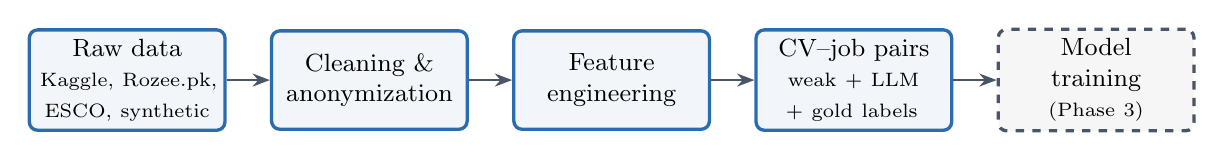
\begin{tikzpicture}[node distance=0.55cm,
  box/.style={draw=rmblue,very thick,rounded corners=3pt,fill=rmblue!6,align=center,
              minimum height=1.25cm,text width=2.25cm,font=\small},
  done/.style={box},
  todo/.style={box,draw=rmgrey,fill=rmgrey!5,dashed},
  arr/.style={-{Stealth[length=2.2mm]},thick,rmgrey}]
\node[done] (raw) {Raw data\\\scriptsize Kaggle, Rozee.pk, ESCO, synthetic};
\node[done,right=of raw] (clean) {Cleaning \&\\anonymization};
\node[done,right=of clean] (feat) {Feature\\engineering};
\node[done,right=of feat] (pairs) {CV--job pairs\\\scriptsize weak + LLM + gold labels};
\node[todo,right=of pairs] (train) {Model\\training\\\scriptsize (Phase 3)};
\draw[arr] (raw) -- (clean);
\draw[arr] (clean) -- (feat);
\draw[arr] (feat) -- (pairs);
\draw[arr] (pairs) -- (train);
\end{tikzpicture}
\caption{Data pipeline. Solid boxes are implemented in this deliverable; model training is Phase~3.}
\end{figure}

\paragraph{Role of external APIs.} Pretrained LLM APIs are used to (i) pre-label CV--job pairs
and generate synthetic CVs for training data, (ii) act as a zero-shot baseline in the
evaluation, and (iii) produce user-facing explanations and rewrites. The retrieval (bi-encoder
\cite{sbert}), reranking (cross-encoder \cite{monobert}) and skill-extraction models are our own
fine-tuned models. Every API call is logged.

\paragraph{Success criteria.} Job and candidate ranking: NDCG@10 and precision@5 on the human
gold set, compared with BM25/TF-IDF and zero-shot LLM baselines. Skill extraction: span-level
F1 against the ESCO dictionary baseline. Bias: change in score under counterfactual swaps of
name, gender, and university should be statistically indistinguishable from zero.

\phase{Phase 2: Data Acquisition \& Preprocessing}

% ---------------------------------------------------------------- 6
\section{Data Collection}
\begin{table}[H]
\centering\small
\begin{tabularx}{\linewidth}{@{}L L l r r@{}}
\toprule
Source & Content & Method & Raw & Clean\\
\midrule
Kaggle \emph{Resume Dataset} \cite{kaggle-resume} & Resume text, 24 job categories & Download & \ResRawMain & \ResFinalMain\\
Kaggle \emph{Updated Resume Dataset} \cite{kaggle-resume2} & Resume text, 25 tech-heavy categories & Download & \ResRawUpd & \ResFinalUpd\\
Kaggle \emph{LinkedIn Job Postings} \cite{kaggle-linkedin} & Title, description, location, level, salary & Download & \JobRawLI & \JobFinalLI\\
Rozee.pk postings & Pakistan-based postings incl.\ skills tags, career level, city & Python scraping & \JobRawRZ & \JobFinalRZ\\
ESCO v1.1.2 skills \cite{esco} & \EscoSkills skills, \EscoAlt alternative labels & Download (CSV) & \EscoSkills & ---\\
Resume--JD fit pairs \cite{hf-fit} & Human-labelled \emph{No / Potential / Good Fit} pairs & Download & \FitPairsTrain\,+\,\FitPairsTest & held out\\
Synthetic CVs & LLM-generated CVs for under-represented roles & API calls (logged) & \multicolumn{2}{r}{script ready}\\
LLM-labelled pairs & \emph{poor / partial / good} labels for built pairs & API calls (logged) & \multicolumn{2}{r}{script ready}\\
\bottomrule
\end{tabularx}
\caption{Data sources with record counts before and after cleaning (Section~\ref{sec:cleaning}).}
\end{table}

\paragraph{Evidence of collection.} Each source has a script in \code{data\_scripts/}:
\code{download\_kaggle.py} (official Kaggle API when credentials exist, otherwise byte-identical
public mirrors on the Hugging Face Hub), \code{download\_esco.py}, \code{scrape\_jobs.py},
\code{generate\_synthetic\_cvs.py}, and \code{label\_pairs.py}. A download manifest records file
names, sizes, row counts and origin. Every LLM call goes through \code{llm\_client.py}, which
appends the prompt, model, response, token usage and timestamp to \code{logs/api\_calls.jsonl}
and caches responses so no call is paid for twice. The client works with any OpenAI-compatible
endpoint (OpenAI, Groq, Gemini).

\paragraph{Scraping policy.} The scraper downloads and obeys \code{robots.txt} for every URL,
waits 2--3\,s between requests (adaptive), sends a descriptive user agent, doubles its delay on HTTP~403/429,
and stores only public posting text (title, company, city, description, skills tags, career
level, experience). It reads structured data from the schema.org \code{JobPosting} block on
each page rather than brittle HTML selectors. Postings were collected for \RozeeQueries of
\RozeeQueriesDefined planned search queries (software, data, design, finance, banking, marketing,
HR and sales). When the site began rate-limiting (\RozeeBlocked of \RozeeRequests requests
answered HTTP~403), the scraper backed off and, after five consecutive blocks, stopped as the
policy requires. The remaining queries (engineering, healthcare, education, internships) are
prioritized automatically on the next run, so the current Pakistani sample is tech-heavy. All requests are
logged to \code{logs/scrape\_rozee.log}. Data is used for academic purposes only; if a site
disallows scraping we rely on Kaggle data for that segment.

\paragraph{Gold set.} \code{sample\_gold\_set.py} draws 200 pairs \emph{only from the test
split} (50\% positives, 30\% hard negatives, 20\% random negatives; pair type hidden from
annotators). Two members label them independently using written guidelines, and the script
reports Cohen's $\kappa$ (plain and linearly weighted) and flags disagreements for
adjudication. This set is never used for training.

% ---------------------------------------------------------------- 7
\section{Data Cleaning Implementation}\label{sec:cleaning}
All cleaning is implemented in Python (pandas, regex, scikit-learn) in
\code{data\_scripts/clean\_resumes.py} and \code{clean\_jobs.py}, with shared utilities in
\code{common.py}. Table~\ref{tab:cleaning} lists each step and its measured effect.

\begin{table}[H]
\centering\small
\begin{tabularx}{\linewidth}{@{}l L r r@{}}
\toprule
Issue & Handling & Resumes & Postings\\
\midrule
Loaded & All sources merged into one schema & \ResRaw & \JobRaw\\
Missing values & Drop records with empty text or title. Fill missing categorical fields
(location, seniority, work type) with \code{unknown}. Salary is never a model input; it is
normalized to yearly values for analysis and left as NaN when missing (\JobSalaryShare\% available). & $-$\ResEmpty & $-$\JobEmpty\\
Encoding noise & Repair mis-decoded UTF-8 (``Na\~{A}\textasciimacron{}ve'' $\rightarrow$ ``Na\"{i}ve''), NFKC normalization & \ResMojibake fixed & ---\\
Noise & Strip HTML tags and entities, URLs, EEO/legal boilerplate, non-printable characters & all & all\\
Non-English & Stop-word ratio test (English vs.\ Spanish/French/German/Portuguese) & $-$\ResNonEn & $-$\JobNonEn\\
Exact duplicates & SHA-1 hash of normalized text & $-$\ResExactDup & $-$\JobExactDup\\
Near-duplicates & TF-IDF cosine similarity $>0.95$ (reposted postings, copied CV templates) & $-$\ResNearDup & $-$\JobNearDup\\
Outliers & Flag below 1st / above 99th percentile of word count (IQR fences as cross-check:
\ResIQR / \JobIQR flagged). Drop clear junk (resumes $<$50, postings $<$30 words); truncate long texts at the 99th percentile & $-$\ResJunk; \ResLong capped & $-$\JobJunk; \JobLong capped\\
Personal data & Replace emails, phone numbers, URLs and street addresses with
\code{[EMAIL]}, \code{[PHONE]}, \code{[URL]}, \code{[ADDRESS]} before any storage or API call
(optional spaCy NER for names) & \ResPII masked & \JobPII masked\\
\midrule
\textbf{Final} & & \textbf{\ResFinal} & \textbf{\JobFinal}\\
\bottomrule
\end{tabularx}
\caption{Cleaning steps and their measured effect (records removed or modified).}\label{tab:cleaning}
\end{table}

\noindent Notable findings: the \emph{Updated Resume Dataset} is mostly duplicates (\ResExactDupUpd
of its \ResRawUpd rows), and the Kaggle resumes still contained real-looking phone numbers and
addresses (\ResPIItokens tokens masked), so anonymization is necessary rather than precautionary.
Removed near-duplicate pairs are saved for inspection, not silently discarded.

% ---------------------------------------------------------------- 8
\section{Feature Strategy}\label{sec:features}
Implemented in \code{data\_scripts/build\_features.py} and \code{skills.py}. All fitted
transformers (scaler, encoder, TF-IDF vocabulary) are fitted on the \emph{training split only}.
\begin{itemize}
\item \textbf{Text normalization:} lowercasing, punctuation cleanup and light rule-based
lemmatization for the TF-IDF baseline only; transformer inputs keep original casing and punctuation.
\item \textbf{Text representations:} TF-IDF over unigrams and bigrams (\TfidfVocab features,
sublinear TF) as the baseline, and 384-dimensional L2-normalized sentence embeddings from
\code{all-MiniLM-L6-v2} \cite{sbert}, to be fine-tuned in Phase~3.
\item \textbf{Skill extraction and normalization:} a gazetteer of ESCO preferred and alternative
labels plus curated tech synonyms maps variants (``JS'', ``ReactJS'', ``k8s'') to one canonical
skill. Ambiguous single words are excluded. This yields on average \MeanSkillsRes skills per
resume and \MeanSkillsJob per posting, and is the baseline the Phase~3 NER model must beat.
\item \textbf{Encoding:} resume categories and posting categories (posting titles mapped to the
same 24 categories by ordered rules, covering \JobCatCov\% of postings) are label-encoded in a
shared label space; skills are multi-hot encoded (\code{MultiLabelBinarizer}) over a vocabulary
of \SkillVocab ESCO skills seen in at least five training documents.
\item \textbf{Numeric features:} text length, number of skills, and years of experience. Years
are extracted by regex from explicit mentions (``5+ years of experience'') or, for resumes, from
the span of dated job entries, with ``Current'' anchored to the collection year of the source
(\RefYear) rather than today (coverage: \YearsCovRes\% of resumes, \YearsCovJob\% of postings).
Heavy-tailed counts are log-transformed, missing years get a train-median value plus a missing
indicator, and all are standardized with \code{StandardScaler}.
\item \textbf{Pair construction:} for each resume, positives are the 3 most similar postings of
the same category; hard negatives are the 2 most similar postings of a \emph{different}
category; one random different-category posting is added. This gives \Pairs pairs
(\PairsPos positive, \PairsHard hard negative, \PairsRand random negative), balanced 50/50.
\item \textbf{Splits:} 70/15/15 train/validation/test split \emph{by resume and by posting}
(not by pair), stratified by category, and pairs are only formed within a split, so no resume
or posting leaks across splits. Resumes: \ResTrain / \ResVal / \ResTest. Postings: \JobTrain /
\JobVal / \JobTest. Pairs: \PairsTrain / \PairsVal / \PairsTest.
\end{itemize}

% ---------------------------------------------------------------- 9
\section{Exploratory Data Analysis}\label{sec:eda}
All charts are produced by \code{data\_scripts/eda.py} on the cleaned data.

\begin{figure}[H]
\centering
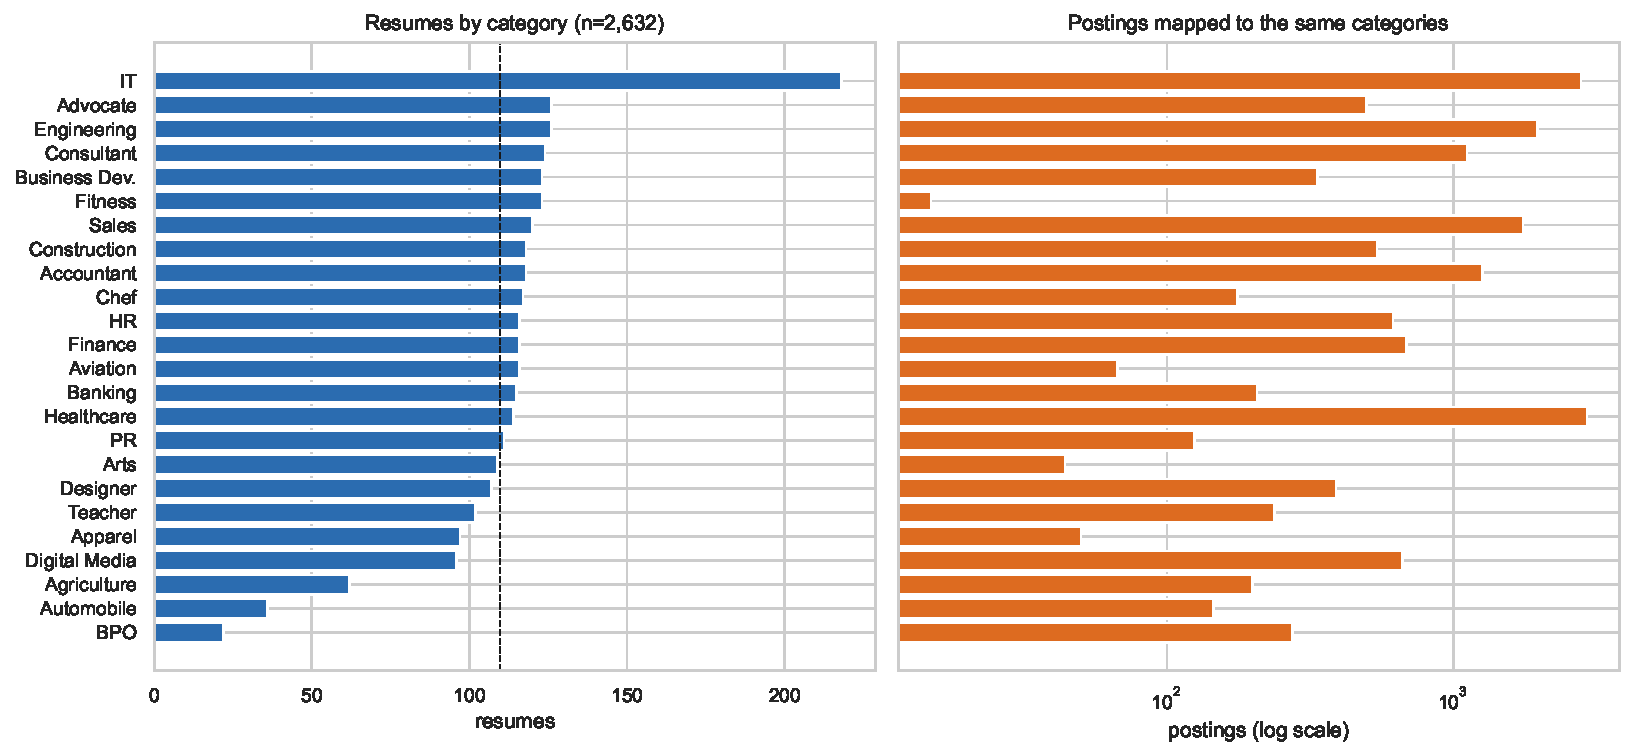
\includegraphics[width=0.86\linewidth]{figures/fig_category_distribution.pdf}
\caption{Class distribution of resume categories (left) and postings mapped to the same
categories (right, log scale). Most resume classes hold 100--125 samples, but the imbalance ratio is
\ImbalanceRatio (\ResCatMax: \ResCatMaxN vs.\ \ResCatMin: \ResCatMinN), so we will use class
weights, stratified splits and synthetic CVs for the rare roles.}
\end{figure}

\begin{figure}[H]
\centering
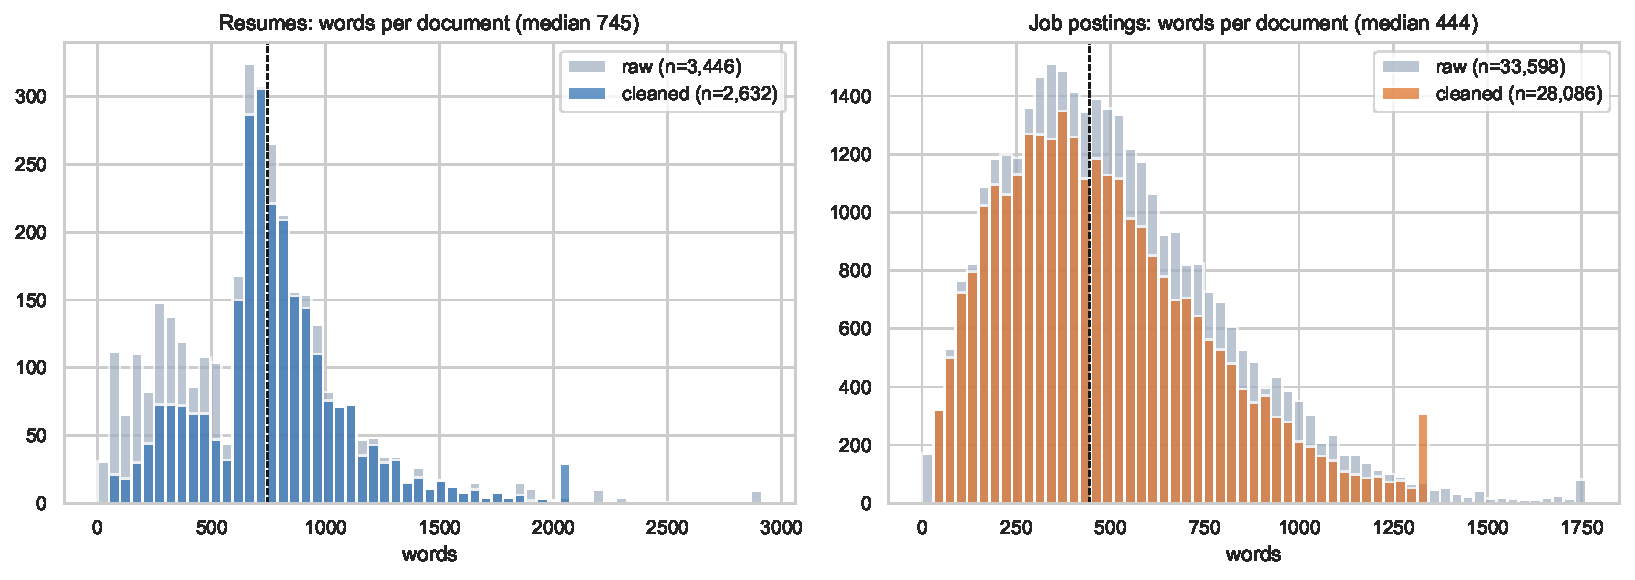
\includegraphics[width=\linewidth]{figures/fig_length_distribution.pdf}
\caption{Text length before (grey) and after cleaning. The median resume has \MedWordsRes words
and the median posting \MedWordsJob. Most short raw resumes disappear because they are
duplicates; the spike at the right edge of the posting histogram is the 99th-percentile cap.}
\end{figure}

\begin{figure}[H]
\centering
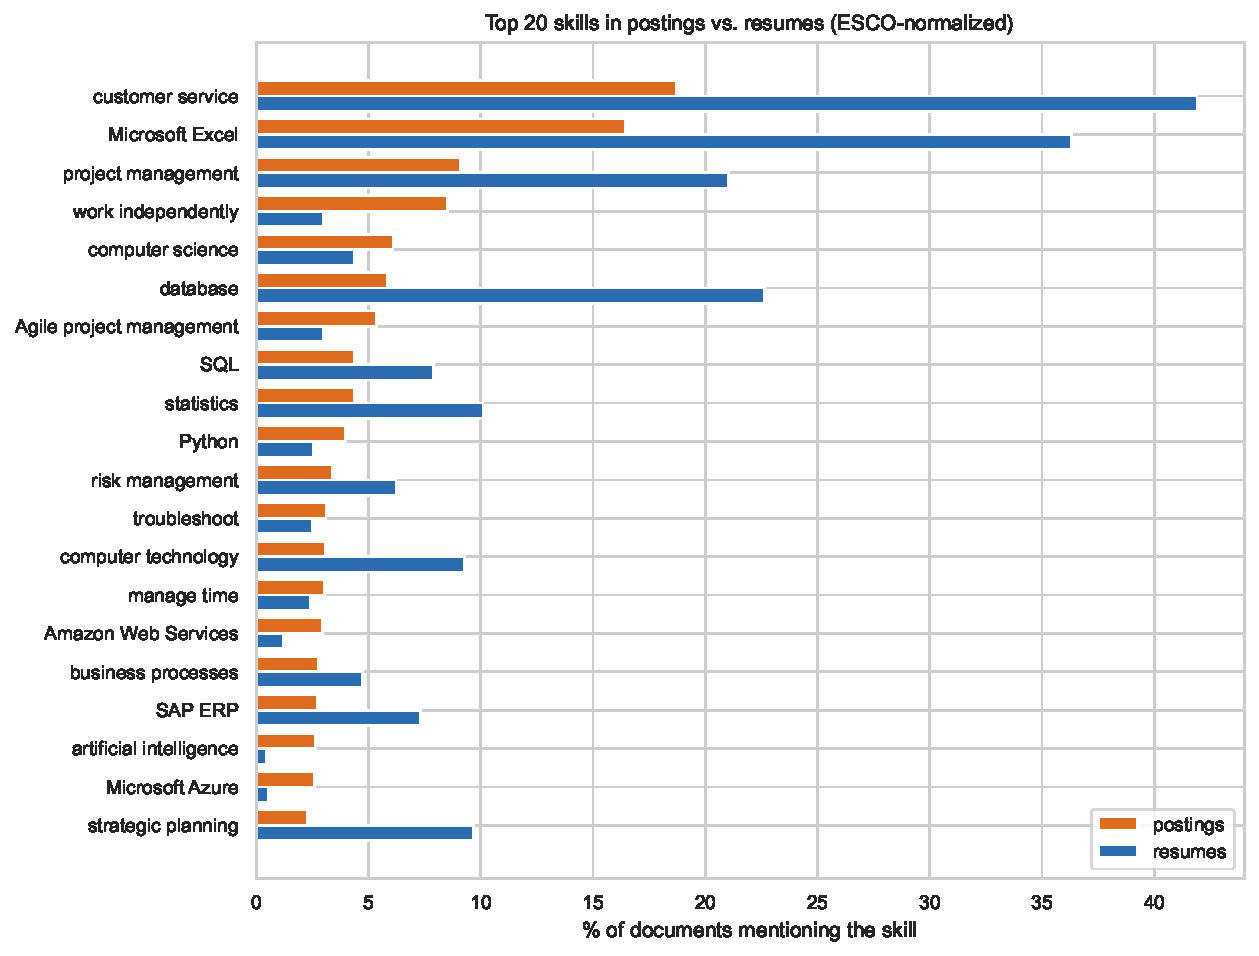
\includegraphics[width=0.82\linewidth]{figures/fig_top_skills.pdf}
\caption{Top 20 skills in postings versus resumes. Resumes over-emphasize generic skills
(customer service, Excel), while postings ask for cloud, AI and Agile skills that resumes rarely
mention. Of the \SkillsUniqJobs distinct skills found in postings, \SkillsJobOnly never occur
in any of the \ResFinal resumes (Jaccard overlap of the two vocabularies: \SkillsJaccard), and
\TopHundredMissing of the 100 most requested skills appear in fewer than 1\% of resumes: the
vocabulary mismatch the skill-gap report targets.}
\end{figure}

\begin{figure}[H]
\centering
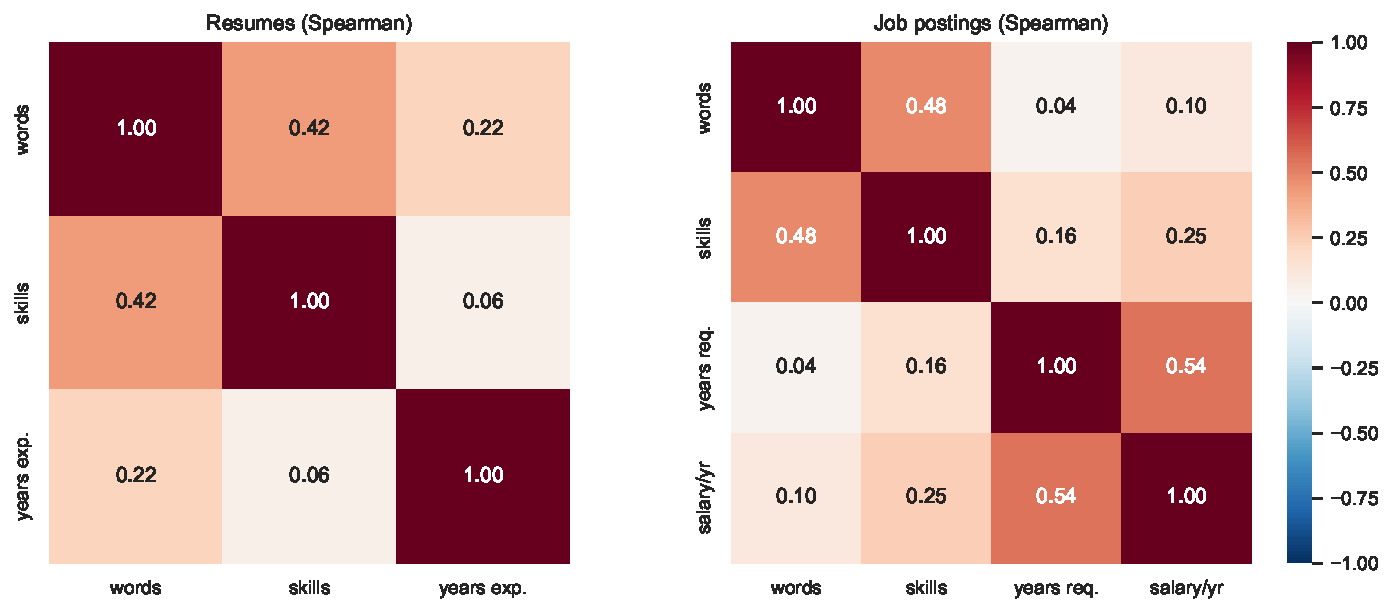
\includegraphics[width=0.92\linewidth]{figures/fig_correlation.pdf}
\caption{Spearman correlations of numeric features. Longer documents list more skills
($\rho=\CorrWordsSkillsRes$ for resumes, \CorrWordsSkillsJob for postings), and required years of
experience is the strongest correlate of advertised salary ($\rho=\CorrYearsSalary$). No pair is
collinear enough to drop a feature.}
\end{figure}

\begin{figure}[H]
\centering
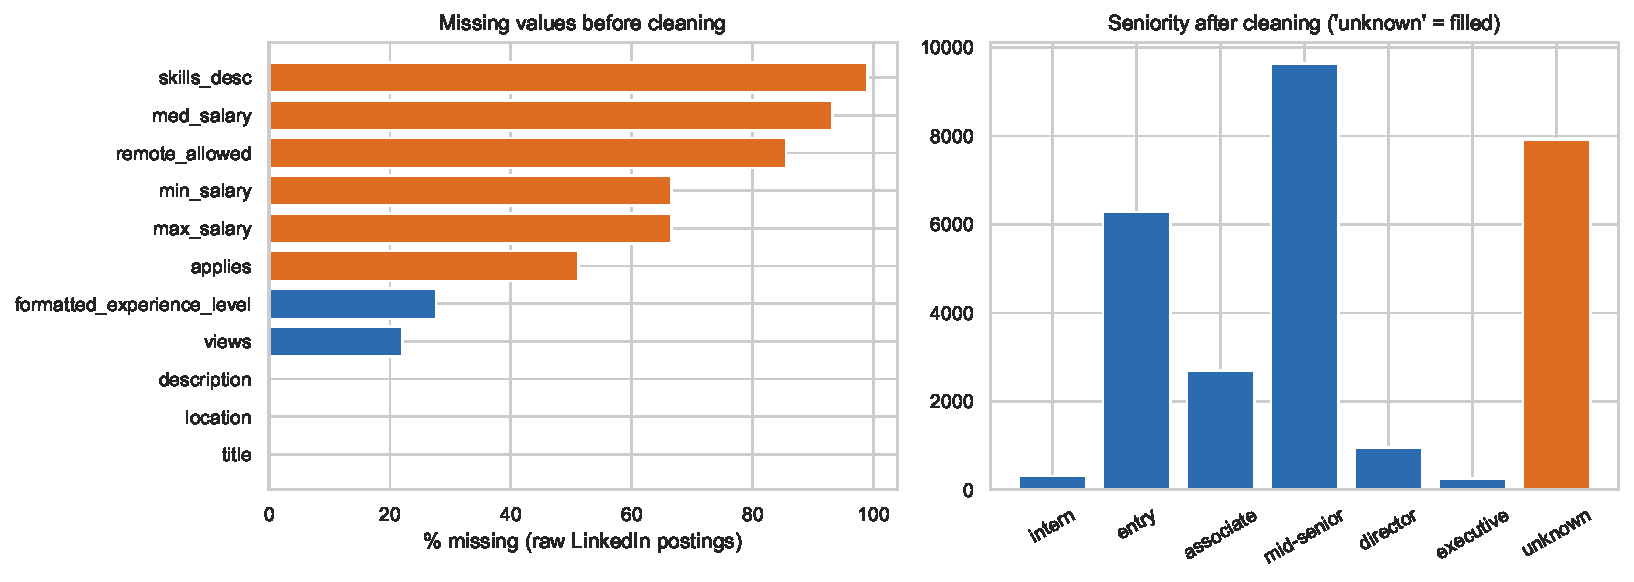
\includegraphics[width=\linewidth]{figures/fig_missing_seniority.pdf}
\caption{Missing values in the raw LinkedIn data (left) and seniority after cleaning (right).
Salary is missing for most postings and is therefore not a model input; \JobSenMissPct\% of
seniority labels are missing and are filled with \code{unknown} instead of being guessed.}
\end{figure}

\begin{figure}[H]
\centering
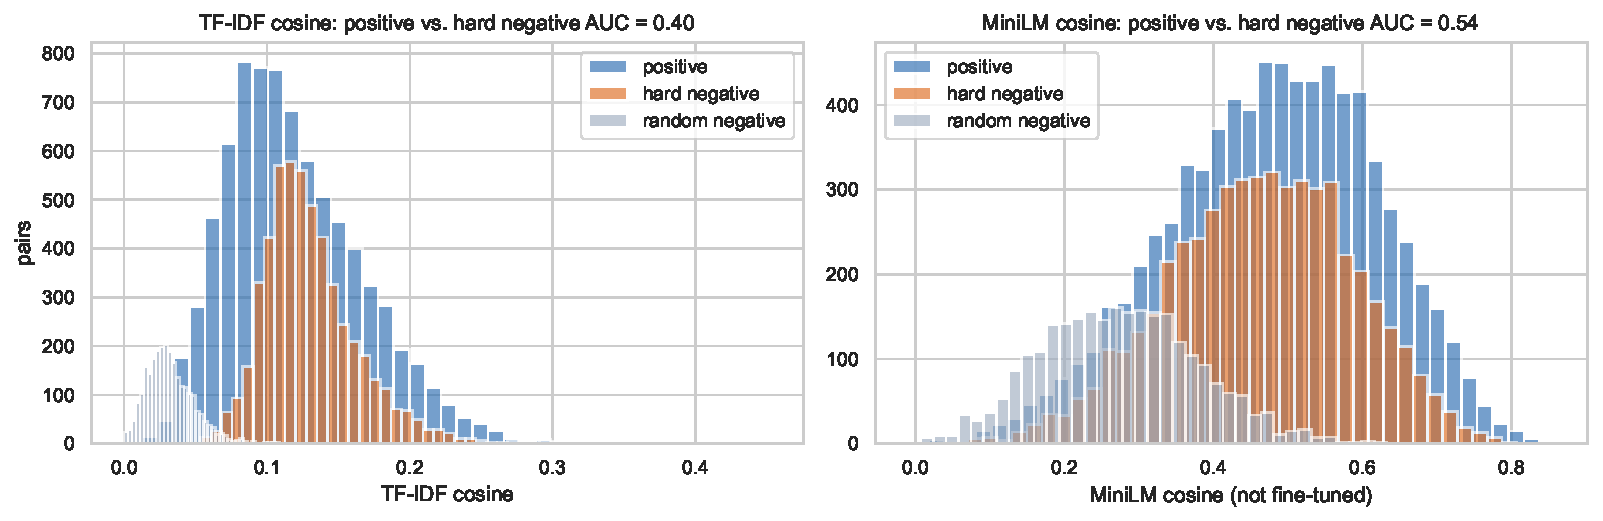
\includegraphics[width=\linewidth]{figures/fig_pairs.pdf}
\caption{Similarity of constructed pairs under TF-IDF (left) and the pretrained, not yet
fine-tuned MiniLM encoder (right). Random negatives are easy to separate, but hard negatives
overlap almost completely with positives (MiniLM mean cosine \EmbHard vs.\ \EmbPos; AUC
\AucEmb). These pairs are exactly the training signal the Phase~3 rankers need.}
\end{figure}

\paragraph{Further observations.} (1) The Kaggle resumes are written by experienced
professionals (median well above ten years of experience), while our primary users are fresh
graduates; synthetic entry-level CVs and the Pakistani postings address this domain gap. (2) The
LinkedIn postings are US-based. The Rozee.pk data adds local titles, cities and skill tags; its
most requested skills are \RozeeTopSkills. (3) \RozeeGendered of the \JobFinalRZ Rozee.pk postings
state an explicit gender preference (\RozeeMale male, \RozeeFemale female). We keep this field
for the Phase~4 bias analysis and never use it as a model input.

% ---------------------------------------------------------------- 10
\section{Repository Structure}
\begin{verbatim}
resumatch/
|-- README.md               # setup, pipeline, data sources
|-- Makefile                # make data scrape clean features eda gold report
|-- requirements.txt
|-- .env.example            # LLM / Kaggle keys (real .env is git-ignored)
|-- .gitignore              # excludes raw data, models, API keys, API cache
|-- data_scripts/
|   |-- common.py           # paths, noise removal, PII masking, dedup helpers
|   |-- download_kaggle.py  # Kaggle API or HF mirrors + manifest
|   |-- download_esco.py
|   |-- scrape_jobs.py      # Rozee.pk, robots.txt-aware, rate-limited
|   |-- llm_client.py       # OpenAI-compatible client, JSONL logging + cache
|   |-- generate_synthetic_cvs.py   # API, logged
|   |-- label_pairs.py              # API, logged
|   |-- clean_resumes.py
|   |-- clean_jobs.py
|   |-- skills.py           # ESCO gazetteer: extraction + normalization
|   |-- build_features.py   # features, splits, pairs, embeddings
|   |-- sample_gold_set.py  # gold set sampling + Cohen's kappa
|   `-- eda.py
|-- data/                   # raw/ interim/ processed/ gold/ (git-ignored)
|-- logs/                   # api_calls.jsonl, scrape log
|-- notebooks/
|-- report/                 # LaTeX source, figures, stats, PDF build
`-- app/                    # Phase 5 (Streamlit/Gradio)
\end{verbatim}

% ---------------------------------------------------------------- 11
\section{Status and Next Steps}
\begin{table}[H]
\centering\small
\begin{tabularx}{\linewidth}{@{}L l@{}}
\toprule
Item & Status\\
\midrule
Kaggle resumes and postings, ESCO taxonomy downloaded & Done\\
Rozee.pk scraper with robots.txt, rate limiting and logging & Done (\JobRawRZ postings)\\
Cleaning, anonymization, deduplication, outlier handling & Done\\
Skill gazetteer, TF-IDF, multi-hot, numeric features, MiniLM embeddings & Done\\
Leakage-free splits and \Pairs weakly labelled pairs & Done\\
EDA figures & Done\\
Synthetic CVs and LLM pair labels (scripts and logging ready) & Pending API key\\
Gold set: 200 pairs sampled; double annotation and $\kappa$ & Pending manual labelling\\
\bottomrule
\end{tabularx}
\caption{Deliverable 1 status.}
\end{table}

% ---------------------------------------------------------------- 12
\section{Risks and Mitigations}
\begin{table}[H]
\centering\small
\begin{tabularx}{\linewidth}{@{}l L@{}}
\toprule
Risk & Mitigation\\
\midrule
Scraping blocked or disallowed & robots.txt checked per URL; fall back to Kaggle postings; keep the scraper limited to permitted pages.\\
Noisy weak / LLM labels & Hand-verify a sample, report agreement, and keep the gold test set human-labelled.\\
Small or imbalanced resume data & Synthetic CVs for rare roles, class weighting, stratified splits.\\
Domain gap (US, senior CVs vs.\ Pakistani graduates) & Rozee.pk postings, synthetic entry-level CVs, separate evaluation on local data.\\
Bias in data (gender, name, institution) & PII anonymized; posting gender preferences kept for auditing only; counterfactual swap tests in Phase~4.\\
API cost or rate limits & All responses cached; a small, cheap model for bulk labelling; exponential back-off.\\
Limited compute & Small models (MiniLM-class) trainable on a free Colab GPU.\\
\bottomrule
\end{tabularx}
\end{table}

% ---------------------------------------------------------------- 13
\section{Team Contribution Plan}
\begin{table}[H]
\centering\small
\begin{tabularx}{\linewidth}{@{}l L@{}}
\toprule
Member & Responsibility in Deliverable 1\\
\midrule
Muhammad Sufyan & Repository setup, scraping scripts, data cleaning pipeline, report\\
{[Member 2]} & Kaggle data cleaning review, EDA, gold-set annotation (annotator 1)\\
{[Member 3]} & Feature engineering, synthetic CV generation, gold-set annotation (annotator 2)\\
\bottomrule
\end{tabularx}
\end{table}

% ---------------------------------------------------------------- refs
\begin{thebibliography}{9}\small
\bibitem{kaggle-resume} snehaanbhawal (Kaggle user). \emph{Resume Dataset}. Kaggle.
\url{https://www.kaggle.com/datasets/snehaanbhawal/resume-dataset}
\bibitem{kaggle-resume2} gauravduttakiit (Kaggle user). \emph{Resume Dataset
(UpdatedResumeDataSet.csv)}. Kaggle. \url{https://www.kaggle.com/datasets/gauravduttakiit/resume-dataset}
\bibitem{kaggle-linkedin} arshkon (Kaggle user). \emph{LinkedIn Job Postings (2023--2024)}. Kaggle.
\url{https://www.kaggle.com/datasets/arshkon/linkedin-job-postings}
\bibitem{hf-fit} \emph{resume-job-description-fit}. Hugging Face Datasets.
\url{https://huggingface.co/datasets/cnamuangtoun/resume-job-description-fit}
\bibitem{esco} European Commission. \emph{ESCO: European Skills, Competences, Qualifications
and Occupations}, v1.1.2. \url{https://esco.ec.europa.eu}
\bibitem{sbert} N.~Reimers and I.~Gurevych. Sentence-BERT: Sentence Embeddings using Siamese
BERT-Networks. \emph{EMNLP}, 2019.
\bibitem{monobert} R.~Nogueira and K.~Cho. Passage Re-ranking with BERT. arXiv:1901.04085, 2019.
\end{thebibliography}

\end{document}
